\documentclass{article} % For LaTeX2e
\usepackage{nips15submit_e,times}
\usepackage{hyperref}
\usepackage{graphicx}
\usepackage{amsmath}
\usepackage{amsthm}
\usepackage{graphicx}
\usepackage{caption}
\usepackage{subcaption}
\usepackage{lmodern}
\usepackage{titlesec}
\usepackage{longtable}
\usepackage{geometry}
\usepackage{multirow}
\usepackage{listings}
\usepackage{amsfonts}
\usepackage{algorithm}
\usepackage{algpseudocode}
\usepackage{multirow}
\usepackage{array}
\usepackage{url}

\author{
Thomas Nedelec \\
MSc Machine Learning\\
\texttt{thomas.nedelec.15@ucl.ac.uk} \\
\And
Michal Daniluk \\
MSc Machine Learning\\
\texttt{michal.daniluk.15@ucl.ac.uk} \\
}
\title{Supervized Learning: Assignment 1}




\newcommand{\fix}{\marginpar{FIX}}
\newcommand{\new}{\marginpar{NEW}}

\nipsfinalcopy % Uncomment for camera-ready version

\begin{document}


\maketitle

\section{Exercise 1: Least Square Regression: effect of the training set size}
We generated a noisy random data set, containing 600 samples, as $y_i = x_i'w + n_i$, where each $x_i$ and $n_i$ are drawn from the standard normal distribution. We splited the data into a training set of size 100 a test set of size 500. We train a linear regression model by Least Square Regression. To evaluate the model, we compute the mean squared error on both the training and test sets. Figure \ref{fig:lsr} shows examples of different training sets and estimated regression $w$.

 \begin{figure}[h]
\center
\begin{tabular}{ccc}
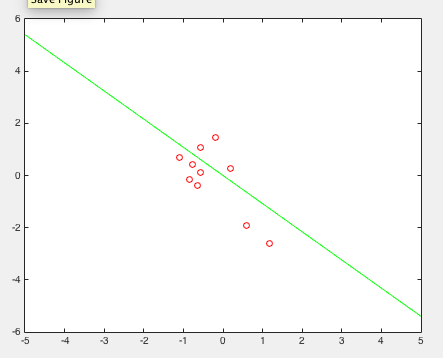
\includegraphics[width=0.3\textwidth]{10points}&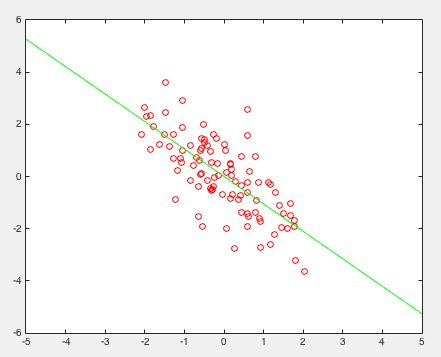
\includegraphics[width=0.3\textwidth]{100points}&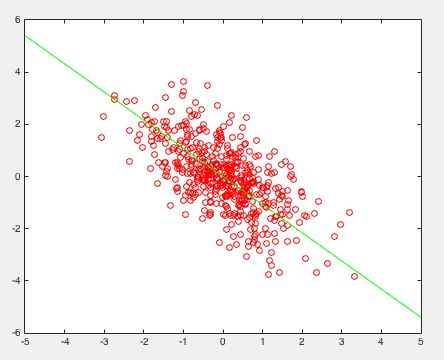
\includegraphics[width=0.3\textwidth]{500points}
\end{tabular}
\caption{ (a) training set of 10 points (b) training set of 100 points (c) the entire data set}
\label {fig:lsr}
\end{figure} 

\begin{figure}[h]
\begin{center}
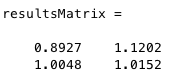
\includegraphics[width=0.3\textwidth]{resultsMatrix}
\caption{Average mean square error for both training and test sets, on both 10 and 100 element-size training set with running 200 times the algorithm.}
\label{fig:resultMatrix1}
\end{center}
\end{figure}


Figure \ref{fig:resultMatrix1} illustrates the ''2 x 2'' table of averages mean square error for both training and test sets, on both 10 and 100 element-size training set. The average mean square run is computed with running 200 times the algorithm. 
\\
We can observe that increasing the size of training set lets to decrease the average mean error on the test set. Indeed, a larger training set lets us to have more information on the distribution and lets to a better generalization of the model. With a small dataset, we do not have enough points to predict well datas in the test set.  
However, it increased the average mean error on train set because it is harder to have a line explaining all the data points.
With increasing the size of training set, the average error on the test and train set becomes similar: the train set is big enough to predict well the test set. The average error on test set will remain a little bit higher than on the train set: normal because it is easy to predict the values of the training set: we have already seen them.

\section{Exercise 2: Least Square Regression: effect of dimensionality}
We repeated the task of exercise 1, but with 10-dimensional data sets. Figure \ref{fig:resultMatrix2} illustrates the ''2 x 2'' table of averages mean square error for both training and test sets, on both 10 and 100 element-size training set.
\begin{figure}[h]
\begin{center}
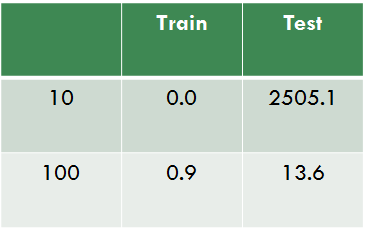
\includegraphics[width=0.4\textwidth]{resultsMatrix2}
\end{center}
\caption{Average mean square error for 10-dimensional data for both training and test sets, on both 10 and 100 element-size training set with running 200 times the algorithm.}
\label{fig:resultMatrix2}
\end{figure}

For 10-sample training set, we obtain the average mean square error $0$ for train set and $2505.1$ for test set. We have 10-dimensional data and 10 samples, so we can accurately predict $y_i$ without any errors. However, the prediction is overfitted to the training data and we have a large error for test set. Increasing number of samples to 100 helps to decrease average error on test set because the biggest size of the training set lets to a better generalization ability. Average error for train set is not anymore 0 because we can't find a space of dimension 10 containing 100 points (except if they only form a 10-dimension space of course).

\section{Exercise 3: Ridge regression}

The regularization is a way to reduce the freedom of the classifier in order to improve the generalization and reach a better test set average error. 
\\ To implement ridge regression, we would like to minimize according to \textit{w} the cost function, 
\begin{equation*}
\gamma w^{T}w + \frac{1}{l} \sum_{i=1}^{l}(x_{i}^{T}w - y_{i})^{2}.
\end{equation*}
Using the notation $X=(x_{1}, x_{2},...,x_{l})^{T}$, a matrix containing the training sample vectors as its rows, we can rewrite the cost function as: 
\begin{equation*}
\gamma w^{T} w + \frac{1}{l} Tr((Xw - Y)^{T}(Xw - Y))
\end{equation*}
Taking derivative according to w, we reach: 
\begin{equation}
2\gamma w + 2 \frac{1}{l} (X^{T}Xw - 2Y^{T}X)=0
\end{equation}
To reach the conditions for optimality, we set the previous equation to zero and we reach: 
\begin{equation}
w=(\gamma l Id +X^{T}X)^{-1}Y^{T}X
\end{equation}
because if $\gamma*l \ne 0$, $(\gamma l Id +X^{T}X)$ is non-singular.

$\gamma l Id +X^{T}X $ is symetric.

We consider $u \in \mathbb{R}^{d}$:
\begin{align*}
\langle (\gamma l Id +X^{T}X)u,u \rangle &= \langle \gamma l u,u \rangle + \langle X^{T}X,u \rangle
\\  &= \gamma l \langle  u,u \rangle + \langle X u, X u \rangle
\\ &= \gamma l ||u||^{2} + ||Xu||^{2} > 0 \textit{ for u $\ne$ 0}
\end{align*}
Thus $\gamma l Id +X^{T}X$ is definite positve. 

\section{Effect of the regularisation parameter}
In this exercise we perform ridge regression on the data sets with the regularisation parameter ranging from $10^{-6}$ up to $10^3$.
First, the graph \ref{fig:ex4_100} shows the training error and test error in function of gamma for 100 training samples. If gamma is too high, the training error and test error increase dramatically. It is intuitive because when gamma is high the algorithm is far more likely to minimize $||w||$  rather than the training error.

 \begin{figure}[h]
\center
 \begin{subfigure}[b]{0.45\textwidth}
        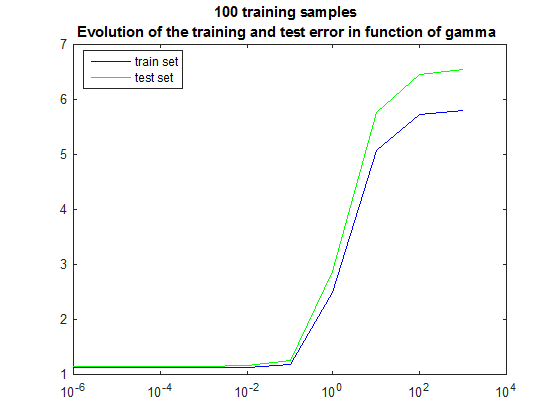
\includegraphics[width=\textwidth]{4_100}
        \caption{One run.}
    \end{subfigure}
    \begin{subfigure}[b]{0.45\textwidth}
        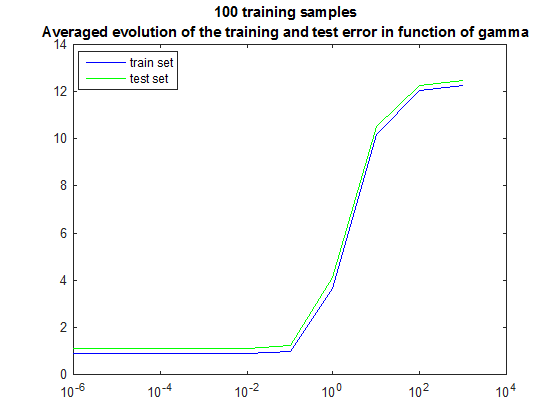
\includegraphics[width=\textwidth]{4_100_avg}
        \caption{Averaged on 200 runs.}
    \end{subfigure}
    \caption{Evaluation of the training error and test error in function of gamma for 100 training samples.}
    \label{fig:ex4_100}
\end{figure}

We have an optimal point corresponding to inflection point of the curve in order to select $\gamma$. Nevertheless, the training set error is not a sufficiently good guidance to select the regularization parameter because the charts are quite different. 

However, when we average the training error on 200 runs, we can observe that now the test error and the training error are now almost identical.
A way to select the optimal $\gamma$ would be to plot the error on the training set averaged on a certain number of runs of the algorithm and select the optimal $\gamma$ on this curve. 

Figure \ref{fig:ex4_10} shows the training error and test error in function of gamma for 10 training samples. 
 \begin{figure}[h]
\center
 \begin{subfigure}[b]{0.45\textwidth}
        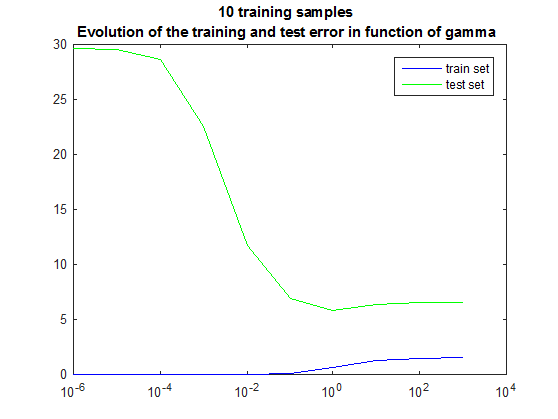
\includegraphics[width=\textwidth]{4_10}
        \caption{One run.}
    \end{subfigure}
    \begin{subfigure}[b]{0.45\textwidth}
        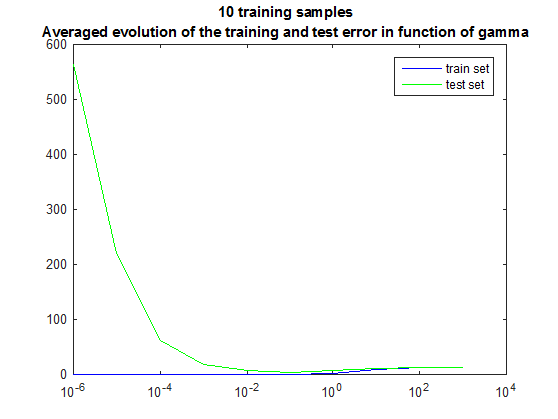
\includegraphics[width=\textwidth]{4_10_avg}
        \caption{Averaged on 200 runs.}
    \end{subfigure}
    \caption{Evaluation of the training error and test error in function of gamma for 10 training samples.}
    \label{fig:ex4_10}
\end{figure}
It looks different than for 100 training samples. Regularization prevented model from overfitting. The test error decreased with increasing regularization parameter until it reached the minimal value for $\gamma = 10^{-1}$. Basically trying to train a regression in dimension 10 with 10 points does not mean a lot of things. However, we can notice some interesting things. 

Regularization prevents algorithm to overfit the data set. In the case of 10 points, it is difficult to choose the optimal value of regularization parameter $\gamma$. Minimizing according to gamma would lead in this case to not take into account the data and choose w=0. T

The most important thing of this part is to see that with a reasonable size of data set there exists an optimal gamma that lets to lead to a good generalization ability. 

\section{Tuning the regularization parameter using a validation set}
The goal of this exercise is to use a validation set to tune the regularization parameter for training set with 10 and 100 samples. Figure \ref{fig:ex5} shows the result error on training, validation and test sets for both data sets.
 \begin{figure}[h]
\center
 \begin{subfigure}[b]{0.45\textwidth}
        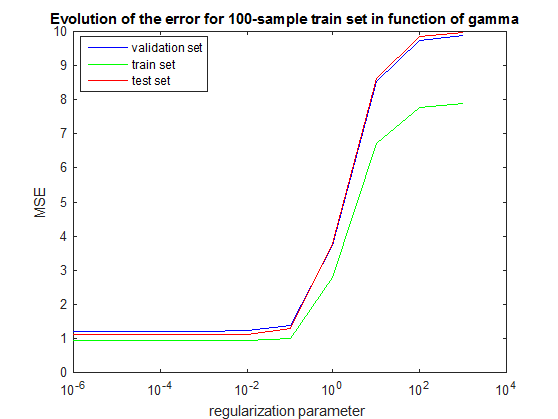
\includegraphics[width=\textwidth]{5_100}
        \caption{100 sample set}
    \end{subfigure}
    \begin{subfigure}[b]{0.45\textwidth}
        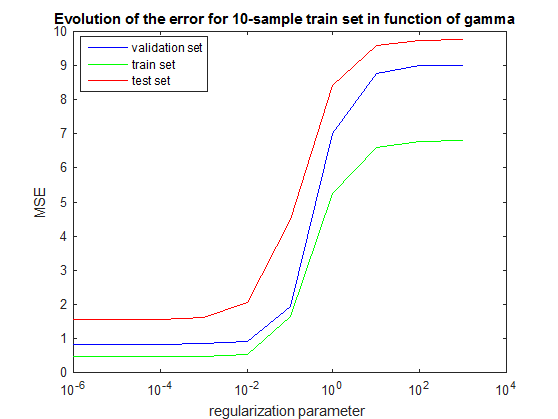
\includegraphics[width=\textwidth]{5_10}
        \caption{10 sample set}
    \end{subfigure}
    \caption{Average MSE in function of gamma .}
    \label{fig:ex5}
\end{figure}

For 100 sample data set, the averaged validation error is almost identical as averaged test error, so it is a good approximation of the error on the test set. The drawback of this method is that we are losing information on the training data because we are only considering 4/5 of the data available to train our regression. 

The averaged best $\gamma$ on the validation set for 200 experiments are : $\gamma^{(100)} = 0.0417 $ and  $\gamma^{(10)} = 50.1787$. The averaged  $\gamma^{(10)}$ is much bigger than  $\gamma^{(100)}$. It is still because with only 10 points, ridge regression just leads to not take into account the training data. Notice that the training set has only 8 samples and the dimension is 10, so we have even less points than dimensions.

We performed RR on the full training set with 100 samples selecting the regularization parameter that gives rise to the smallest validation set error.Training error and validation error are equal to $0.2027$ and $3.2162$ respectively for 10 sample set and   $0.8513$ and $1.1106$  for 100 sample set. It's obvious that for bigger training set we reached better results.

It is better to tune regularization parameter on validation set, which is independent from training set but we are losing information compare to having access to the full training set. That is why we need to introduce cross-validation. 

\section{Tuning the regularization parameter using cross validation}
We use 5-fold cross validation to tune the regularization parameter. Figure \ref{fig:ex6} shows cross-validation score on top of the training and test set error for different values $\gamma = \{10^{-6}, 10^{-5}, \dots, 10^3 \}$ of the regularization parameter.

\begin{figure}[h]
    \centering
    \begin{subfigure}[b]{0.3\textwidth}
        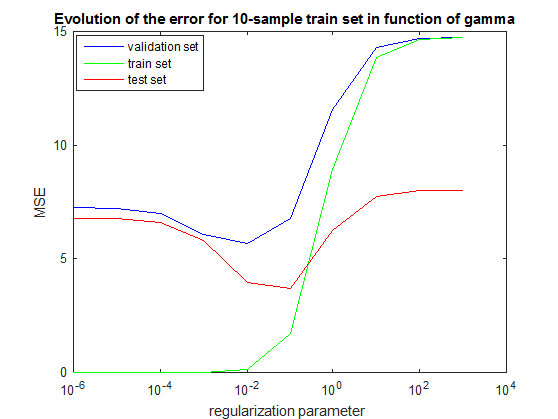
\includegraphics[width=\textwidth]{ex6_10}
        \caption{10-sample training set}
    \end{subfigure}
    \begin{subfigure}[b]{0.3\textwidth}
        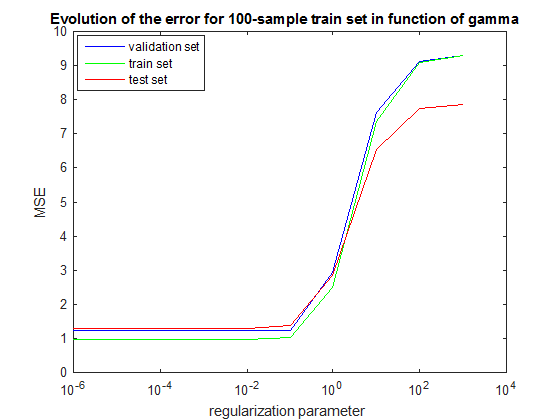
\includegraphics[width=\textwidth]{ex6_100}
        \caption{100-sample training set}
    \end{subfigure}
    \caption{Evaluation of the mean square error in function of gamma for different number of training examples.}
    \label{fig:ex6}
\end{figure}

\newpage
Cross validation error is a good estimation of error for test set for both 100 samples and we do not lose anymore data in the training set. 



\section{Comparison of  $\gamma$ tuning methods}
The goal of this exercise is to generate 200 such data as in above exercises and tune the regularization parameter $\gamma$ using three methods. The results of average test error and standard deviation of the errors for 10 sample set-up are presented below:

\begin{enumerate}
\item By minimizing the training error
\begin{itemize}
\item Test set error: $163.9892$
\item Standard deviation of error: $508.3517$
\end{itemize}
\item By minimizing the validation error (80\% / 20 \% split)
\begin{itemize}
\item Test set error: $35.5974$
\item Standard deviation of error: $192.3498$
\end{itemize}
\item By minimizing the 5-fold cross validation error
\begin{itemize}
\item Test set error: $6.2890$
\item Standard deviation of error: $10.1677$
\end{itemize}
\end{enumerate}

The best results gives tuning regularization by minimizing the 5-fold cross validation error. Minimizing the 5-fold cross validation error gives us reasonable results despite the fact that training set size is very small. Minimizing the training error doesn't seem to be a good approach, because the test set error and  standard deviation of error are very big. Indeed we do not have enough information to hope to predict well on the test set. Using only one validation set gives us better results but still not such as good as using cross validation method. Indeed in the validation set method, we are losing information compare to cross-validation methods.

The results of average test error and standard deviation of the errors for 100 sample set-up are presented below:

\begin{enumerate}
\item By minimizing the training error
\begin{itemize}
\item Test set error: $1.1202$
\item Standard deviation of error: $0.0831$
\end{itemize}
\item By minimizing the validation error (80\% / 20 \% split)
\begin{itemize}
\item Test set error: $ 1.1529$
\item Standard deviation of error: $ 0.1283$
\end{itemize}
\item By minimizing the 5-fold cross validation error
\begin{itemize}
\item Test set error: $1.1208$
\item Standard deviation of error: $0.0848$
\end{itemize}
\end{enumerate}
First of all, the results are much better than for 10 sample set-up. We increased the size of the training set and now our model has a good generalization ability. Secondly,  differences between results for each method are very small. It's because, we have a big enough train set and regularization isn't really necessary. We still can notice that cross validation is better than validation because thanks to cross-validation we do not need to loose information compare to cross-validation. 

\section{Load the data}
We loaded the boston data set into Matlab.
\section{Baseline versus full linear regression.}
In this exercise we try a baseline method works for a problem instead of use all of our attributes for prediction. Firstly, we implemented Naive Regression, (approach whose name is well chosen..) which predicts with the mean y-value on the training set. The averaged training and test errors (after 20 runs) are equal to $ 84.5706$ and $84.3933$ respectively. 

Then Linear Regression with single attributes was implemented. For each of the thirteen attributes, we performed a linear regression using only the single attribute but incorporating a bias term. Results are shown in figure \ref{fig:res}. 

In general, results are better than for Naive Regression, but they depend on which attribute we selected. It means that some attributes are more important (have more information that we can use to distinguish classes) that others. For example, Linear Regression with 13th attribute has error on test set: $39.1051$ in contrast to with 4th attribute: $83.5478$. 

Linear Regression using all attributes outperforms obviously any of the individual regressors (MSE on test set: $27.8889$.


\section{Kernel Ridge Regression}
In this exercise we will perform kernel ridge regression on the Boston data set with the Gaussian kernel, which is defined as:
\begin{equation*}
K(x_i,x_j) = exp(-\frac{|| x_i - x_j||^2}{2 \sigma^2})
\end{equation*}

First, we compute the kernel matrix for all the data (when we implement cross-validation we select indexes which are meaningful for the training set and validation set). 

Then, we used \textit{kridgereg.m} to perform kernel ridge regression using equation $\alpha^* = (K + \gamma l I_l)^{-1}y$. We don't explicitly use a matrix inverse instead use the matrix left division operator. According to the Matlab documentation, \textit{mldivide} is a more efficient way to solve a linear equation $Ax = b$. If the solution does not exist or if it is not unique, the  \textit{mldivide} operator issues a warning.

Then, we created a function called \textit{dualcost.m} to calculate the Mean Squared Error (MSE) using equation:
\begin{equation}
mse = \frac{1}{l}(K_{test} \alpha - y)'(K_{test} \alpha - y)
\end{equation}

We perform kernel ridge regression on the training set using five-fold cross-validation with different values of $\gamma$ and $\sigma$. Figure \ref{fig:ex910} shows the cross-validation error as a function of $\gamma$ and $\sigma$. 
\begin{figure}[h]
    \centering
    \begin{subfigure}[b]{0.45\textwidth}
        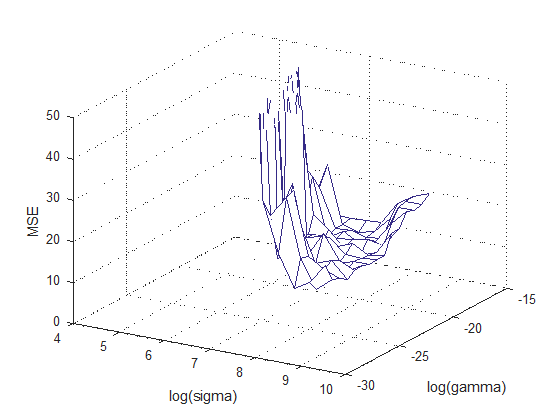
\includegraphics[width=\textwidth]{ex910_1}
    \end{subfigure}
    \begin{subfigure}[b]{0.45\textwidth}
        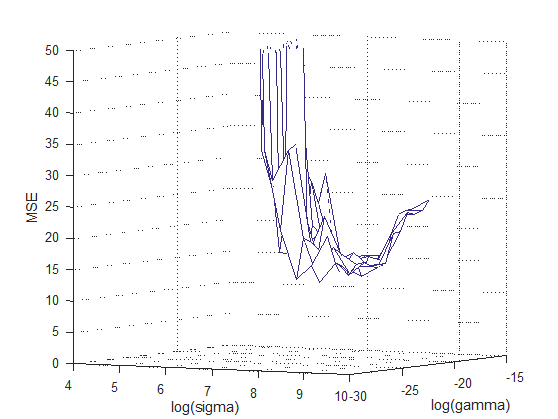
\includegraphics[width=\textwidth]{ex910_2}
    \end{subfigure}
    \caption{Cross-validation error as a function of $\gamma$ and $\sigma$.}
    \label{fig:ex910}
\end{figure}
The best results are for values $\gamma = 2^{-31}$ and $\sigma = 2^{12}$. The MSE on the training data $= 8.8392$ and on the test set $= 13.8215$.

Then, we repeat those steps over 20 random splits of data. Our results for exercise 9 and 10 are summarized in the table:
\begin{center}
\begin{tabular}{|  l c r|}
  \hline
  \textbf{Method} & \textbf{MSE train} & \textbf{MSE test} \\
  Naive Regression & 84.5706 $ \pm $ 3.7489 & 84.3933 $ \pm $ 7.3810\\
 Linear Regression (attribute 1) & 71.9206 $ \pm $ 3.7157& 71.7623$ \pm $ 7.2524\\
  Linear Regression (attribute 2) & 73.4863 $ \pm $ 4.2998& 73.7122$ \pm $ 8.4777\\
 Linear Regression (attribute 3) & 64.8467 $ \pm $ 4.6972& 64.7529$ \pm $ 9.1959\\
 Linear Regression (attribute 4) & 81.3032 $ \pm $ 3.2466& 83.5478$ \pm $ 6.3118 \\
 Linear Regression (attribute 5) & 69.1346 $ \pm $ 3.6979& 69.0250$ \pm $ 7.8448\\
 Linear Regression (attribute 6) & 43.0045 $ \pm $ 4.6585& 45.4416$ \pm $ 9.3804\\
 Linear Regression (attribute 7) & 72.6169 $ \pm $ 4.3741& 72.4109$ \pm $ 8.5975\\
 Linear Regression (attribute 8) & 79.1138 $ \pm $ 4.3852& 79.6780$ \pm $ 8.5893\\
 Linear Regression (attribute 9) & 72.4303 $ \pm $ 4.2039& 71.9495$ \pm $ 8.2573\\
 Linear Regression (attribute 10) & 66.3728 $ \pm $ 4.5274& 65.3491$ \pm $ 8.9139\\
 Linear Regression (attribute 11) & 63.3372 $ \pm $ 3.9821& 61.7821$ \pm $ 7.9450\\
 Linear Regression (attribute 12) & 75.1591 $ \pm $ 3.8102& 75.1225$ \pm $ 7.5406\\
  Linear Regression (attribute 13) & 38.2716 $ \pm $ 2.1729& 39.1051$ \pm $ 4.2303\\
  Linear Regression (all attributes) & 23.1232 $ \pm $ 2.9711& 27.8889$ \pm $ 6.2950\\
 Kernel Ridge Regression  & 7.9308$ \pm $1.3363 & 13.7928$ \pm$ 2.4398\\
  \hline
\end{tabular}
 \label{fig:res}
\end{center}
\section{Part 2}
\subsection{Simulating \texitt{1-Nearest Neighbor classifier} with Linear Classifier}

According to the previous part, 
\begin{equation*}
\alpha^{*}=(K+\gamma*l*I_{l})^{-1}y
\end{equation*}
If $\beta$ is big, $K_{\beta}(x,t)=exp(-\beta*||x-t||^2)=0$ if x is very different from t and not equal to zero if x is close from t. If $\beta$ is really too big everything is equal to if x different from t. Thus, there is an optimal beta to try to consider the closest point with a linear classifier.

\subsection{Using a perceptron to learn a linear classifier with a bias}
\begin{equation*}
f_{w,b}(x)=sign(w^{T}x+b)
\end{equation*}
To learn also the bias, we use the algorithm presented in different articles: 
\begin{algorithm} [H]
\caption{Perceptron}
\\Input $D: training set, maxIter, learningRate$ 
\begin{algorithmic} [1]
\State $w_d\gets 0$
\\initialize w=0, $b_{0}=0$, k=0
\\$R=max\{||x_{i}||, 1 \leq i \leq l\}$
 \\While mistakes are made in the for loop repeat:
 \For{$iter = 1 \dots l$}
		\If {$y_{i}(w_{k}^{T}x_{i}+b_{k}  \le 0$} 
   		     \State $w_{k+1}=w_{k}+\eta*y_{i}x_{i}$
		     \State $b_{k+1}=b_{k}+\eta*y_{i}R^{2}$
		     \State k=k+1
  		 \EndIf
	 \EndFor
 \EndFor
 \State\Return{ $w_d$}
\end{algorithmic}
\end{algorithm}


\end{document}
